\documentclass[border=4pt]{standalone}
\usepackage{tikz}
\usetikzlibrary{positioning, arrows.meta, shapes.geometric, calc, fit, backgrounds}
\usepackage{amsmath}
\begin{document}
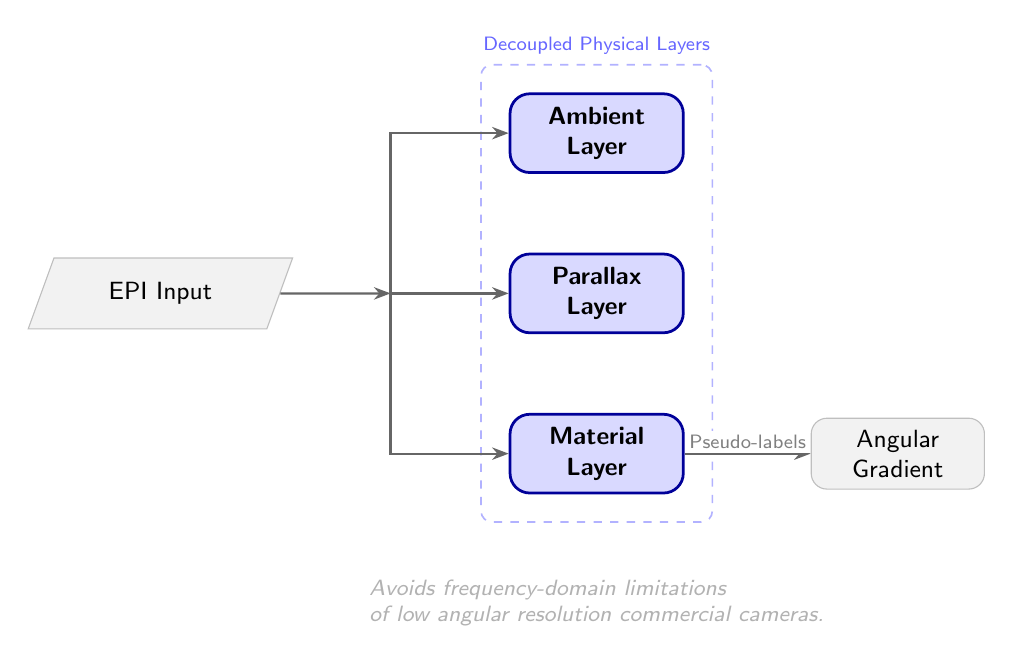
\begin{tikzpicture}[
  node distance=1.0cm and 1.5cm,
  input/.style={draw, trapezium, trapezium left angle=70, trapezium right angle=110,
                minimum width=1.8cm, minimum height=0.9cm,
                fill=gray!10, draw=gray!50, align=center, font=\sffamily\small},
  innov/.style={draw, rounded corners=2.5mm, minimum width=2.2cm, minimum height=1.0cm,
                fill=blue!15, draw=blue!60!black, line width=1pt, align=center,
                font=\sffamily\small\bfseries},
  output/.style={draw, rounded corners=2mm, minimum width=2.2cm, minimum height=0.9cm,
                 fill=gray!10, draw=gray!50, align=center, font=\sffamily\small},
  arr/.style={-{Stealth[length=6pt]}, thick, color=black!60},
  lbl/.style={font=\sffamily\scriptsize, text=black!50, fill=white, inner sep=1.5pt},
  gbox/.style={draw=blue!30, dashed, rounded corners=4pt, inner sep=10pt, line width=0.6pt},
  note/.style={font=\sffamily\footnotesize\itshape, text=gray!60, align=left},
]

% Input
\node[input] (m1) {EPI Input};

% Split point
\coordinate[right=1.4cm of m1.east] (split);

% Decoupled Layers
\node[innov, right=1.5cm of split] (m3) {Parallax\\Layer};
\node[innov, above=1.0cm of m3] (m2) {Ambient\\Layer};
\node[innov, below=1.0cm of m3] (m4) {Material\\Layer};

% Output
\node[output, right=1.6cm of m4] (m5) {Angular\\Gradient};

% Arrows
\draw[arr] (m1) -- (split);
\draw[arr] (split) |- (m2);
\draw[arr] (split) -- (m3);
\draw[arr] (split) |- (m4);
\draw[arr] (m4) -- node[lbl, above] {Pseudo-labels} (m5);

% Grouping
\begin{scope}[on background layer]
  \node[gbox, fit=(m2)(m3)(m4),
        label={[font=\sffamily\scriptsize, text=blue!60]above:Decoupled Physical Layers}] (group) {};
\end{scope}

% Annotation
\node[note, below=0.6cm of group.south, anchor=north, align=left]
  {Avoids frequency-domain limitations\\of low angular resolution commercial cameras.};

\end{tikzpicture}
\end{document}